\documentclass[12pt,oneside]{sotsuken_paper}

% タイトル
\title{超低重心6輪独立懸架ローバーの画像情報による自律走行}
\author{佐々井翔也・戸澗健・畠中和久}

\begin{document}
% 行間
\setlength{\baselineskip}{9truemm}

%文字間
\kanjiskip=.53zw plus 3pt minus 3pt
\xkanjiskip=.53zw plus 3pt minus 3pt

% 目次
\tableofcontents
%\newpage

% 本文

\chapter{緒言}
\section{研究の背景}

\subsection{前年度のロボットの問題点}
%そこで今回は走破性の向上を考え,前年度の改善案として低重心化とそれを補佐する懸架装置に注目し,”超低重心6輪独立懸架ローバー”を制作する
前年度,つくばチャレンジで使用したロボットの重心が高かったため,凸凹道やコンクリートなどでロボットが傾きそのまま転倒する恐れがあった.
そのため,前年度の問題点を元に転倒しても走行可能なロボットの開発を試みた.だが,今年度のつくばチャレンジに参加するにあたり,ロボットの高さ制限を満たし,転倒しても走行可能な機構の開発ができなかった.
よって今回はロボットの走破性を高めることで,転倒しにくいロボットの開発を行った.
\subsection{自己位置の推定}
ロボットが自律走行を行うためには,自身の位置を推定する必要がある.
その手段としてローカルマップをグローバルマップに変換する方法が主流である.
これはロボットが何らかの方法で周辺の情報を得る必要があり,一般的に測域センサや地磁気センサが用いられることが多い.
また,近年はカメラを用いた信号認識など視覚情報を用いた研究が活発である.
そこで今回は低コストで省スペース化が期待できる単眼カメラを用いることにした.
\subsection{三角測量とカメラの移動量}
ローカルマップを生成するために周囲との位置関係を求める必要がある.
カメラでは対象物を写した2枚の画像とそれらの画像間距離から三角測量の原理を用いることで対象物からカメラまでの距離を計測することができる.以下にその原理を図\ref{fig:sankaku1}として示す。図のように三角測量を行う際には2つのカメラを用いるのが一般的だ.だが今回はカメラを移動させ過去の位置で取得した画像を利用することで単眼カメラで三角測量を行えるようにした.この原理を図\ref{fig:sankaku2}に示す.図\ref{fig:sankaku2}より,カメラ間の距離はカメラの移動量に等しい.よってカメラの移動量を取得することができれば対象物との位置関係が分かる.

\section{研究の目的}
今年度は走破性の向上を考え,前年度の改善案として低重心化とそれを補佐する懸架装置に注目し,”超低重心6輪独立懸架ローバー”を開発する.またカメラの移動量をモーションセンサから得られる位置情報によって取得し,三角測量を行う.これを複数回行い,得られたデータをマップとする.

\section{論文の構成}

\chapter{つくばチャレンジについて}
%\section{つくばチャレンジの概要}
\section{つくばチャレンジの概要}
今年度参加したつくばチャレンジについて説明する.つくばチャレンジとは茨城県南部に位置するつくば市の屋外で行こなわれるロボット実験である.これは人間とロボットの共存する社会の実現のための先端的技術への挑戦が狙いである.人間とロボットの共存を目的とするため,ロボットには以下のことが求められる.
\begin{enumerate}
 \item そこにいる人間が安全であること
\item そこにいる人間に危害を加えないこと.またそのように取られる不安感を与えないこと
 \item 環境内に存在するものに手を加えないこと.また環境景観を損なわない外観であること
\item 環境内に存在するものの邪魔にならないこと.また,環境内の運動を妨害しないこと
\end{enumerate}
これらの項目が満たされていなければつくばチャレンジでは走行を行うことができない.また,つくばチャレンジではその走行に対して課題が与えられる.以下につくばチャレンジのコースを図\ref{fig:tizu}として示す(つくばチャレンジ2016の課題より参照).

\begin{figure}[htp]
 \begin{center}
  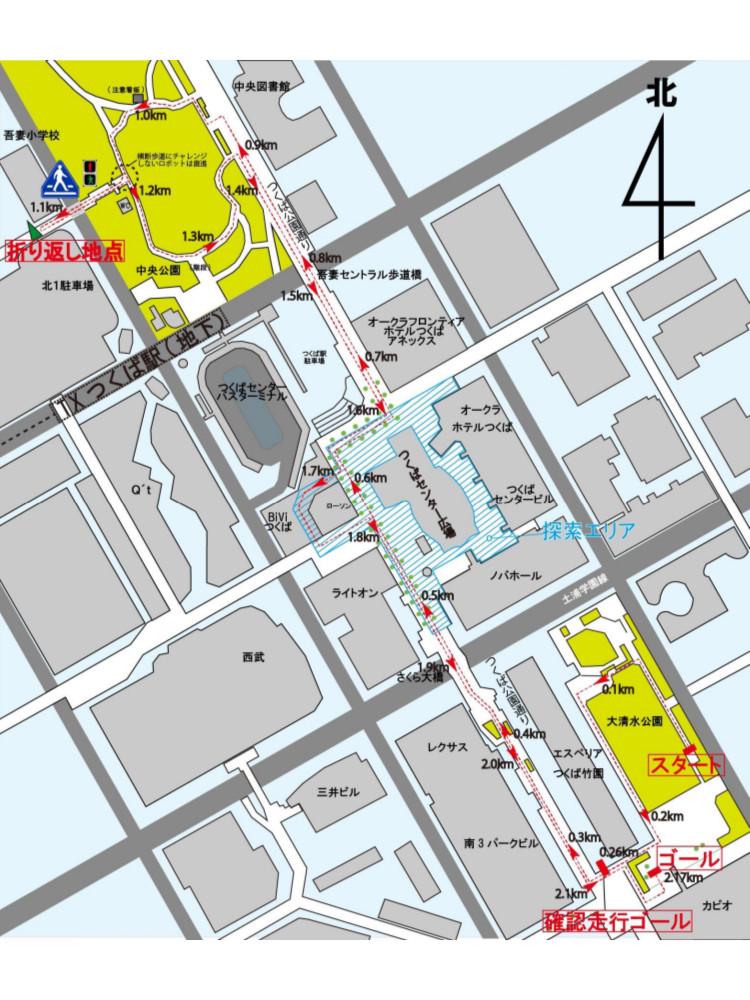
\includegraphics[width=100mm]{img/hard/tizu.jpg}
  \caption{つくばチャレンジコース図}
  \label{fig:tizu}%ここに文章中で使用する名前を指定する
 \end{center}
\end{figure}

\section{今年の課題}
今年度のつくばチャレンジの課題について説明する.全体のコース,コース環境,そしてロボットに必要な機能をそれぞれ述べる.またロボットは歩道橋等を走行するが,その場合原則として端より1m以上離れての走行とされる.
\subsection{全体のコース}
本コースのスタート地点は図\ref{fig:tizu}の右下に位置するつくば市大清水公園東側の歩道をスタート点とし、公園内を反時計回りに周回する.コースは大清水公園から遊歩道へと進み,更に北上してつくばセンター広場へと出る.この広場の東側を探索エリアと呼ぶ.センター広場から北上し,途中左折して中央公園に入り,公園内を反時計回りに周回する.中央公園内の周回途中で,一旦右折して信号機付の横断歩道を渡る.そして北1駐車場脇で折り返し,再度横断歩道を渡り中央公園に戻る.中央公園を周回したあと,再度つくば公園通りの遊歩道に戻り,つくばセンター広場に向かって南下する.センター広場では,西側にあるBiViつくば(つくばバスターミナルビル)の2階の自動扉を通り,その中を通り抜ける.そのまま遊歩道を南下大清水公園に戻る.大清水公園入口のつくばカピオ前がゴールである.

\subsection{コース環境}
本大会のコースはつくば市民が日頃生活をしている生活環境である.したがって日常のように人や自転車が通行している.つくばチャレンジでは危険防止のため安全責任者を各チーム内から定め,ロボットの走行時には通行人や見物人に注意を呼びかける.


ロボットの走行エリアと市民の歩く領域は区別されない.天候は当日の天候状況によるが,小雨程度であれば滞り無く開催される.また路面や環境の状況(落ち葉,水たまりなど)も前日やそれ以前の天候,または社会的条件(お祭りなど)に大きく影響を受ける.


ロボットは環境内にもともと存在する街路樹や縁石柵あるいは建物を走行のガイドとして用いるのは自由であるが,ロボットの走行の為に新しくガイドとなるものを設置することや,環境を改変することは許されない.

\subsection{ロボットに必要な機能}
\chapter{ハードウェアの概要}

\section{ロボットの構成}
今年度のロボットに搭載したセンサを以下の表\ref{tab:op}に示す.

\begin{table}[h]
  \begin{center}
    \caption{ハードウェアの構成}
    \small
  \scalebox{0.85}{
  \begin{tabular}{|c|c|} \hline
    構成要素 & メーカ・型番・スペックなど \\ \hline
    Mian PC & NVIDIA JETSON TK1 \\ \hline
    OS & Ubuntu 14.04 LTS \\ \hline
    camera & Panasonic HX-A1H \\ \hline
    Buttery & KyPOM KT5100 4S 35C \\ \hline
    Motor & MABUCHI MOTOR RS-555VC-5524 \\ \hline
    Motion Sensor & 東京航空計器株式会社 CSM-MG100\\ \hline

  \end{tabular}
  }
    \label{tab:op}
  \end{center}
\end{table}

\section{ロボットの外観}

\section{システムの構成}
\begin{figure}[htp]
 \begin{center}
  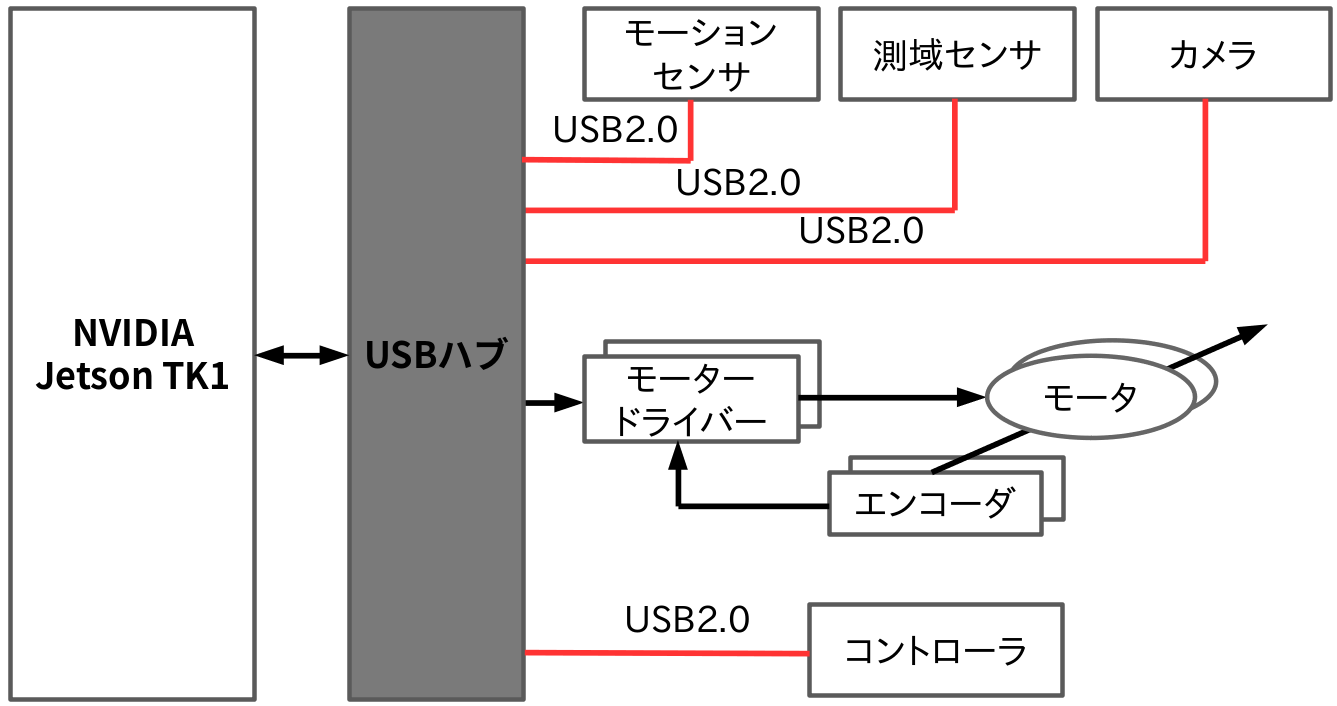
\includegraphics[width=100mm]{img/hard/sisutemu.png}
  \caption{システム構成}
  \label{fig:sisutemu}%ここに文章中で使用する名前を指定する
 \end{center}
\end{figure}

\section{低重心化の実現}
設計した走行モジュールのCADを図\ref{fig:cad}に示す。図から確認できるように全高がタイヤ直径である190mm内に収まっているため低重心化が達成された.また6輪に付属している懸架装置を図\ref{fig:kenka}に示す.ばねを2本設置することでサスペンションとし,またそれらの取り付け位置を斜めにすることでさらに低重心が可能となった.

\begin{figure}[htp]
 \begin{center}
  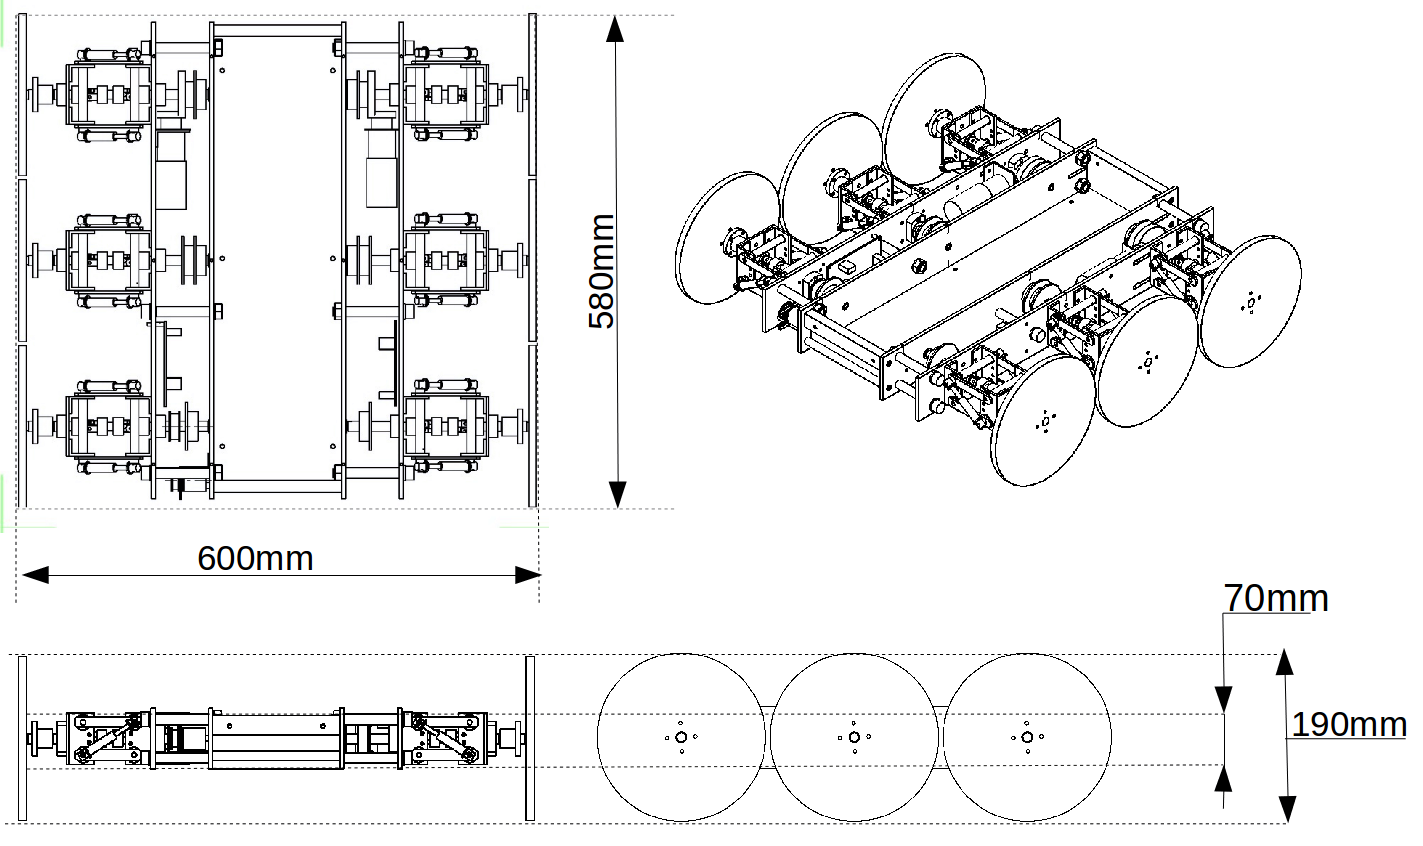
\includegraphics[width=100mm]{img/hard/4.png}
  \caption{走行モジュール}
  \label{fig:cad}%ここに文章中で使用する名前を指定する
 \end{center}
\end{figure}

\begin{figure}[htp]
 \begin{center}
  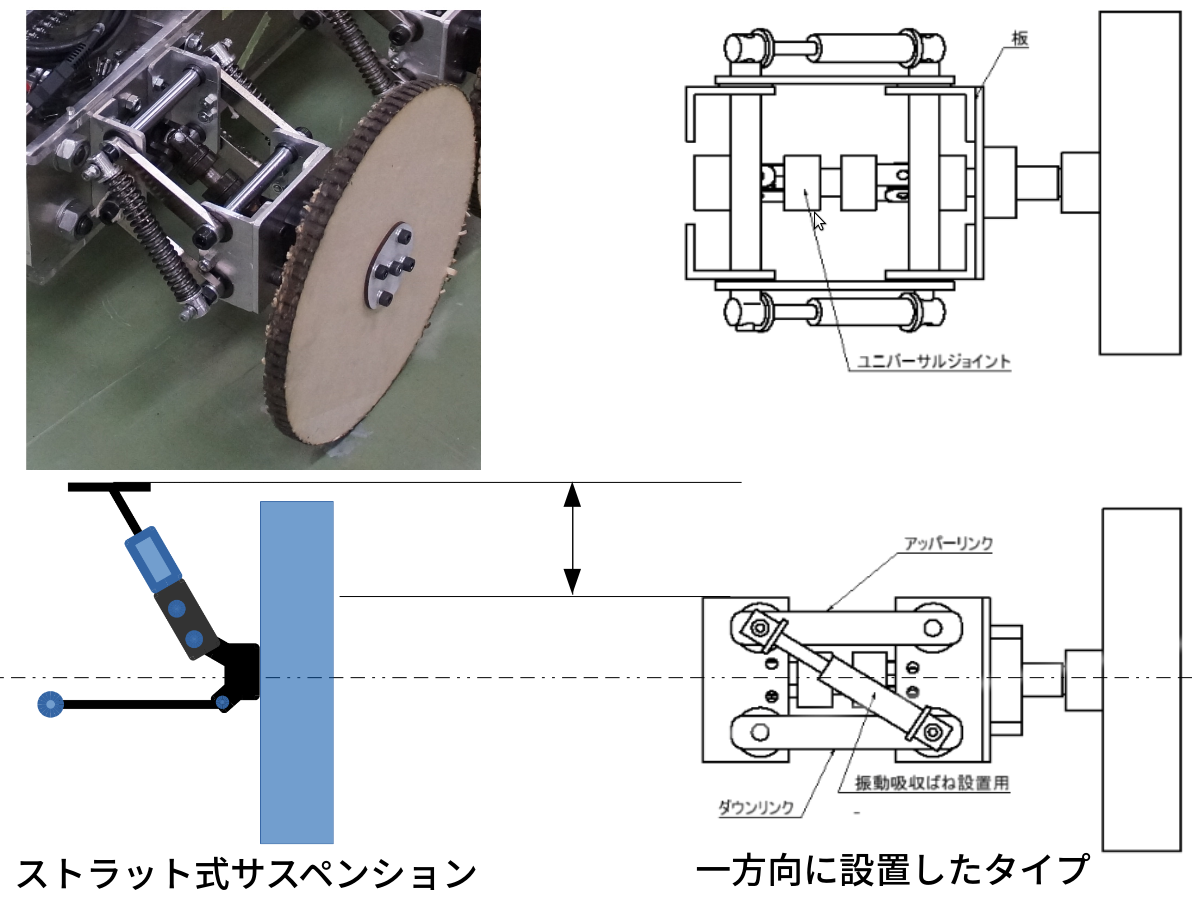
\includegraphics[width=100mm]{img/hard/3.png}
  \caption{懸架装置}
  \label{fig:kenka}%ここに文章中で使用する名前を指定する
 \end{center}
\end{figure}


\section{超堤・超壕能力}
今回作成したロボットの性能を調査するため,超堤・超壕実験を行った結果,超堤:110[mm],超壕220[mm]が得られた.

\chapter{マップ生成}
\section{移動量の取得}
カメラの移動量を取得するため,東京航空計器社製のモーションセンサから得られる位置情報を使用する.モーションセンサーを図\ref{fig:motion}に示す.1回目に取得した位置と2回目に取得した位置の
差から移動量を算出する.

\begin{figure}[htp]
 \begin{center}
  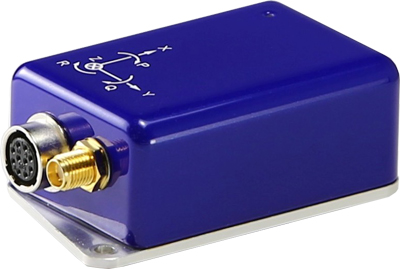
\includegraphics[width=50mm]{img/soft/motion.jpg}
  \caption{モーションセンサー}
  \label{fig:motion}%ここに文章中で使用する名前を指定する
 \end{center}
\end{figure}

\section{マップ生成環境}
マップの生成環境を図\ref{fig:map}に示す.天候はカメラ画像に影響の少ないくもりの日,画像間距離を1.4[m]として金沢工業高等専門学校の駐車場付近でマップ生成を行った.ロボットはStart地点から矢印の方向に進み,2回の旋回を経てGoal地点まで走行する.

\begin{figure}[htp]
 \begin{center}
  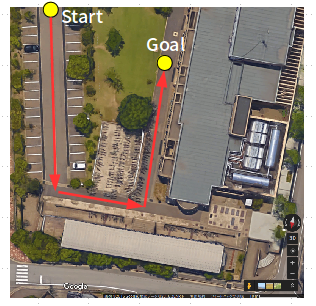
\includegraphics[width=80mm]{img/soft/1.png}
  \caption{マップ生成環境}
  \label{fig:map}%ここに文章中で使用する名前を指定する
 \end{center}
\end{figure}

\section{マップ生成}
生成されたマップを図\ref{fig:mapp}に示す.赤い点群はカメラ画像から三角測量によって得られた周囲の位置関係,青い線はカメラ画像から得られたロボットの走行軌跡,黄色い線を実際にロボットが走行した軌跡である.
図より,カメラ画像からマップを生成することができた.
しかしカメラ画像から得られたロボットの走行軌跡は1回目の旋回時から,実際にロボットが走行した軌跡と比べて大きく歪んでいることが確認できる.

\begin{figure}[htp]
 \begin{center}
  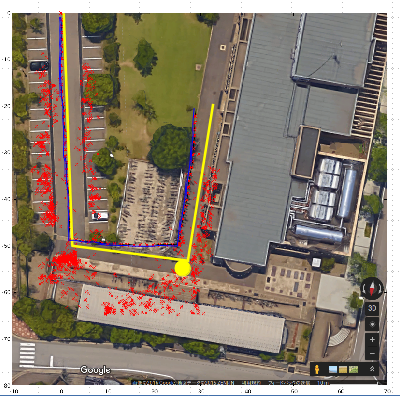
\includegraphics[width=80mm]{img/soft/2.png}
  \caption{生成したマップ}
  \label{fig:mapp}%ここに文章中で使用する名前を指定する
 \end{center}
\end{figure}

\section{移動量のばらつき}
マップ生成を行った際にモーションセンサーから得られた移動量のばらつきを図\ref{fig:gps}に示す.

\begin{figure}[htp]
 \begin{center}
  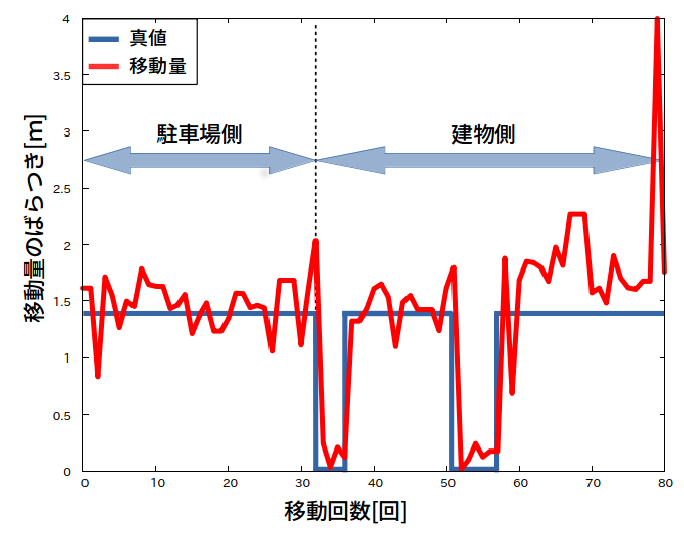
\includegraphics[width=80mm]{img/soft/gps.png}
  \caption{移動量のばらつき}
  \label{fig:gps}%ここに文章中で使用する名前を指定する
 \end{center}
\end{figure}

図を見て分かるとおり,駐車場側では取得した移動量が真値から増減しているためマップ生成をした際のズレが小さい.しかし建物側に近づくに連れて取得した移動量が真値よりも大きく増加してしまっている.また旋回時は移動を行っていないため移動量は0[m]になっている必要があるのに対し,取得した移動量は0[m]になっておらず,これらの原因によってマップ生成の際にズレが発生してしまったと考えられる.

\chapter{結言}
\section{本研究のまとめ}
走破性の高いロボットの開発の実現にあたり,つくば市内での走行が問題なく行えたため,走破性の高いロボットの開発は達成したと考える.また移動量の取得とマップ生成の実現にあたり,生成したマップは旋回時に大きく歪むことが確認されたが直線時には問題がなかったため3次元復元技術の基礎は確立できたと考える.

\section{今後の課題}
\subsection{自己位置推定と自律走行}

\subsection{タイヤ素材検討}

\subsection{屋内対応}
今回我々は移動量を取得するためにGPSから得られる位置情報を使用しているため,GPSを取得することができない屋内などでは移動量を取得することができない.そこで我々が使用したモーションセンサーは位置情報以外にも加速度や姿勢なども取得することができるため,これらのセンサー情報から屋内でも移動量を取得し屋内マップを生成する.

\subsection{全天候性の付与}

% 参考文献
\begin{thebibliography}{8}
%  \bibitem{harris} LandingProducts, APCPro\nolinebreak pellers,\nolinebreak
%http://www.\linebreak apcprop. com{\slash}v{\slash}index.html,
%2012/8/21
%\bibitem{kyonenn} GPS測位計算プログラム入門,ROS,http://www.enri.go.jp/~fks442/K_MUSEN
\bibitem{ros} Bradski,Kaehler:詳解 OpenCV,433,株式会社オライリー・ジャパン(2012)
\bibitem{kyonenn} 理解するためのGPS測位計算プログラム入門,http://www.enri.go.jp/~fks442%/K_MUSEN
%  \bibitem{koukuu} 中村 資郎:新航空工学講座 第7巻 プロペラ:日本航空技術協会,pp.23-24,1988
%  \bibitem{rikigaku} 加藤 寛一郎,大屋 昭男,柄沢 研治:航空機力学入門,東京大学出版会,pp.32,1982
\end{thebibliography}



\chapter*{謝辞}
\addcontentsline{toc}{chapter}{謝辞}
本論文作成にあたりテーマの決定,研究の考え方,方法のまとめ方など全てにおいて長期にわたって厳しくも熱意のあるご指導,ご鞭撻していただいた,伊藤恒平教授に厚く御礼申し上げます.


特に分析においても論文の書き方においても論文を何度も読んでいただき,指導していただいた伊藤恒平教授に大変ご苦労をかけてしまいましたことにも心よりお詫び申し上げたいです.


同級生のメンバーには論文の作成,修正にご協力いただき心より感謝しております.
その他、助けていただいた多くの皆様に心から感謝しております.ありがとうございました.

\end{document}

